%%%%%%%%%%%%%%%%%%%%%%%%%%%%%%%%%%%%%%%%%%%%%%%%%%%%%%%%%%%%%%%%%%%%%%%%
\chapter{Ontwikkelpotentie}
%%%%%%%%%%%%%%%%%%%%%%%%%%%%%%%%%%%%%%%%%%%%%%%%%%%%%%%%%%%%%%%%%%%%%%%%

\begin{center}
  \begin{minipage}{0.5\textwidth}
    \begin{small}
    \end{small}
  \end{minipage}
  \vspace{0.5cm}
\end{center}

%%%%%%%%%%%%%%%%%%%%%%%%%%%%%%%%%%%%%%%%%%%%%%%%%%%%%%%%%%%%%%%%%%%%%%%%
\section{Inleiding}
%%%%%%%%%%%%%%%%%%%%%%%%%%%%%%%%%%%%%%%%%%%%%%%%%%%%%%%%%%%%%%%%%%%%%%%%

Voor de in hoofdstuk 2.4 uitgelichte techieken is er veel data nodig om een realistisch gesynthetiseerde stem met menselijk en persoonlijk karakter te realiseren. In dit hoofdstuk wordt de beschikbaarheid van Nederlandse datasets onderzocht en toegelicht. Ook wordt er een schatting gemaakt over de benodigde kwantiteit en kwaliteit van de data om deze stem te realiseren.


%%%%%%%%%%%%%%%%%%%%%%%%%%%%%%%%%%%%%%%%%%%%%%%%%%%%%%%%%%%%%%%%%%%%%%%%
\section{Beschikbare Nederlandse datasets}
%%%%%%%%%%%%%%%%%%%%%%%%%%%%%%%%%%%%%%%%%%%%%%%%%%%%%%%%%%%%%%%%%%%%%%%%

\subsection{Corpus Gesproken Nederlands (CGN)}
Het Corpus Gesproken Nederlands is door het Instituut voor de Nederlandse Taal in 2014 ontwikkeld \footnote{\url{https://ivdnt.org/downloads/taalmaterialen/tstc-corpus-gesproken-nederlands}}. Deze dataset bevat 900 uur aan Nederlandse spraak, afkomstig van Vlamingen en Nederlanders. Dit maakt de dataset een \textit{multi-speaker} dataset, waarvan de uitdagingen al zijn uitgelijnd in het vorige hoofdstuk. Alle spraakfragmenten, in totaal 12.780, zijn getranscribeerd met orthografische en fonetische transcripties. Ook zijn ze syntaacticsh en met POS-tags (woordsoort informatie) geannoteerd. Het lexicon van deze dataset beslaat ongeveer 9 miljoen woorden. Deze dataset is ontworpen voor het testen van spraakherkennings software. In tabel \ref{tab:cgn} worden zijn alle spraakcategorieën onderverdeeld. Het gebruik van deze dataset is gratis, zowel voor niet-commercieel als commercieel gebruik, alhoewel er een licentie moet worden ondertekend voor het gebruik ervan.

Hoewel er veel goed geannoteerde, Nederlandse spraakdata aanwezig is in deze dataset, heeft deze een zeer heterogene samenstelling waarbij audiokwaliteit, stemkwaliteit, meerdere stemmen, de aanwezigheid van het Vlaams en context een belemmering vormen. Om deze reden is deze dataset niet geschikt om te worden gebruikt voor de eerder genoemde neurale netwerken. Wel is het geschikt als dataset voor een Nederlands speech-to-text systeem.

\begin{table}[]
    \centering
    \scalebox{0.75}{
        \begin{tabular}{l|c|c|c}
            Component & Totaal a. woorden & VL & NL \\
             Spontane conversaties ('face-to-face') & 2.626.172 & 878.383 & 1.747.789 \\
             Interviews met leraren Nederlands & 565.433 & 315.554 & 249.879 \\
             Telefoondialogen opgenomen m.b.v. telefooncentrale & 1.208.633 & 465.096 & 743.537 \\
             Telefoondialogen opgenomen m.b.v. minidiscrecorder & 853.371 & 343.167 & 510.204 \\
             Zakelijke onderhandelingen & 136.461 & 0 &  136.461 \\
             Interviews en discussies uitgezonden op radio en televisie & 790.269 & 250.708 & 539.561 \\
             Discussies, debatten, vergaderingen (m.n. politieke) & 360.328 & 138.819 & 221.509 \\
             Lessen & 405.409 & 105.436 & 299.973 \\
             Spontane commentaren (o.a. sport) uitgezonden op radio en televisie  & 208.399 & 78.022 & 130.377 \\
             Actualiteitenrubrieken en reportages uitgezonden op radio en televisie & 186.072 & 95.206 & 90.866 \\
             Nieuwsbulletins uitgezonden op radio en televisie & 368.153 & 82.855 & 285.298 \\
             Beschouwingen en commentaren uitgezonden op radio en televisie & 145.553 & 65.386 & 80.167 \\
             Missen, lezingen, plechtige toespraken & 18.075 & 12.510 & 5.565 \\
             Colleges, voordrachten, lezingen & 140.901 & 79.067 & 61.834  \\
             Voorgelezen teksten & 903.043 & 351.419 & 551.624  \\
             \textbf{Totaal} & \textbf{8.916.272} & \textbf{3.261.628} & \textbf{5.654.644}
        \end{tabular}
    }
    \caption{Corpus Gesproken Nederlands 	spraakcategorieën}
    \label{tab:cgn}
\end{table}

\subsection{LibriVox}
LibriVox is een website dat audioboeken, in het publieke domein aanbiedt. De boeken zijn ingesproken door vrijwilligers op het platform en zijn, hoewel niet altijd volledig professioneel opgenomen, van adequate kwaliteit om datasets van te maken. LibriVox heeft op het moment van schrijven 287 boeken in het Nederlands beschikbaar gesteld \footnote{\url{https://librivox.org/search?primary_key=19&search_category=language&search_page=1&search_form=get_results}}. Zoals eerder besproken, geniet het samenstellen van een homogene dataset met maximaal 1 stemacteur en veel uren spraakdata de voorkeur. Er zijn een aantal vrijwilligers die meerdere boeken hebben ingesproken, waaronder \textit{Marcel Coenders} met een catalogus van 112 voorgelezen boeken \footnote{\url{https://librivox.org/reader/2450?primary_key=2450&search_category=reader&search_page=1&search_form=get_results}}. In theorie is deze hoeveelheid spraakdata genoeg om een overtuigende stem te verkrijgen door middel van hedendaagse technieken (WaveNet, Tacotron 2).

LibriVox biedt alleen de audio opnames van de boeken aan. Een orthografische transcriptie opgelijnd aan de tekst wordt dus niet aangeboden, deze zal moeten worden samengesteld door middel van speech-to-text software en handmatig werk.

Een nadeel dat wordt genoemd in het gebruik van audioboeken als dataset, is dat de stemacteur vaak op geacteerde wijze de teksten voorleest. Dit heeft zeer mogelijk een impact op de gesynthetiseerde stem, waardoor voor commerciële implementaties gekozen wordt een volledig eigen dataset te maken met neutraal gesproken en gecureerde zinnen.

%%%%%%%%%%%%%%%%%%%%%%%%%%%%%%%%%%%%%%%%%%%%%%%%%%%%%%%%%%%%%%%%%%%%%%%%
\section{Oplijnen orthografische transcriptie}
%%%%%%%%%%%%%%%%%%%%%%%%%%%%%%%%%%%%%%%%%%%%%%%%%%%%%%%%%%%%%%%%%%%%%%%%
Voor deep learning text-to-speech technieken moet de dataset in een vorm worden gezet, zodat het netwerk de latente translatie kan maken tussen tekst en spraak. Doorgaans wordt spraakdata in fragmenten geknipt, waarbij elk audio fragment een apart bestand is en een zin bevat. Naast alle bestanden met audio fragmenten, wordt er ook een lijst bijgehouden van de orthografische transcriptie van de spraak per bestand. Deze lijst bestaat uit de kolommen zoals weergegeven in Tabel \ref{tab:orthografische_file}.

Voor het automatisch oplijnen en genereren van transcripties uit een spraakdata bestand, bevat het bestand ook tijdcodes van de start en eindpositie van de transcriptie in de spraakdata. Deze methode heet \textit{forced alignment}, waarbij audio en tekst met elkaar worden gesynchroniseerd. Een veelgebruikte, open-source software voor deze taak is \texttt{aeneas} \footnote{\url{https://github.com/readbeyond/aeneas}}. Hierbij wordt een bestand gegenereerd zoals aangegeven in Figuur \ref{fig:aenas}. 

\begin{table}[]
    \centering
    \scalebox{0.7}{
        \begin{tabular}{c|c|c}
            bestands naam & orthografische transcriptie & genormaliseerde, orthografische transcriptie \\
            librivox\_1.wav & Dhr. Koenders bestelde 46 tomaten bij de groenteboer. & De heer Koenders bestelde zes en veertig tomaten bij de groenteboer.
        \end{tabular}
    }
    \caption{Kolommen van een orthografisch transcriptie bestand}
    \label{tab:orthografische_file}
\end{table}

\begin{figure}
    \centering
    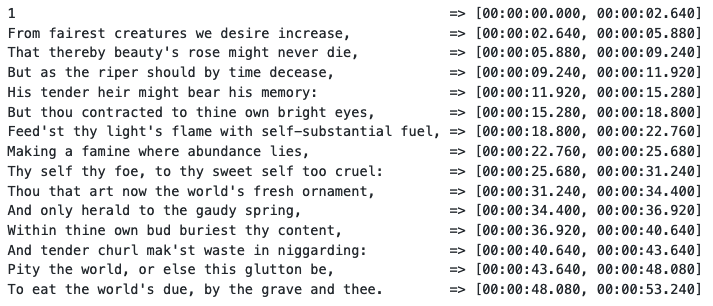
\includegraphics[width=0.75\textwidth]{figures/transcription.png}
    \caption{Voorbeeld bestand van een automatische, orthografische transcriptie met tijdcodes}
    \label{fig:aenas}
\end{figure}


\subsection{LJSpeech}
Hoewel dit een Engelse dataset betreft, wordt deze toch toegelicht door de unieke, homogene samenstelling en segmentatie ervan. LJSpeech is een spraak dataset in het publieke domein van 13.100 korte audio fragmenten van een spreker die passages leest van 7 verschillende non-fictie boeken. De audio fragmenten hebben een lengte van 1 tot 10 seconden, samenvattend bevat het ongeveer 24 uur aan spraak data. Alle audio fragmenten zijn orthografische getranscribeerd, zowel in de geschreven als gezegde (genormaliseerde) vorm. In de genormaliseerde vorm worden cijfers, de aanhef en andere afkortingen volledig uitgeschreven.

Elk audio fragment is een mono, 16-bit PCM WAV bestand met een sample rate van 22050 Hz. De LJSpeech dataset wordt vaak gebruikt in text-to-speech wedstrijden, workshops van conferenties en intern om modellen te testen. Het formaat en de omvang dient daarom als een streven voor het samenstellen van een Nederlandse variant. Ook kan deze dataset worden gebruikt als experiment om hypothesen op te toetsen en, met op het oog het budget, een ontwikkelrichting te maken voor een Nederlands gesynthetiseerde stem.

\begin{table}[H]
    \centering
    \begin{tabular}{c|c}
    Totaal a. fragmenten & 13,100 \\
    Totaal a. woorden & 225,715 \\
    Totaal a. karakters & 1,308,674 \\
    Totale lengte & 23:55:17 \\
    Gemiddelde lengte audio fragment & 6.57 sec \\
    Minimale lengte audio fragment & 1.11 sec \\
    Maximale lengte audio fragment & 10.10 sec \\
    Gemiddeld a. woorden per audio fragment & 17.23 \\
    Unieke woorden & 13,821 \\
    \end{tabular}
    \caption{LJSpeech dataset statistieken}
    \label{tab:ljspeech}
\end{table}


% LJ001-0002|in being comparatively modern.|in being comparatively modern.
% LJ001-0003|For although the Chinese took impressions from wood blocks engraved in relief for centuries before the woodcutters of the Netherlands, by a similar process|For although the Chinese took impressions from wood blocks engraved in relief for centuries before the woodcutters of the Netherlands, by a similar process
% LJ001-0004|produced the block books, which were the immediate predecessors of the true printed book,|produced the block books, which were the immediate predecessors of the true printed book,
% LJ001-0005|the invention of movable metal letters in the middle of the fifteenth century may justly be considered as the invention of the art of printing.|the invention of movable metal letters in the middle of the fifteenth century may justly be considered as the invention of the art of printing.
% LJ001-0006|And it is worth mention in passing that, as an example of fine typography,|And it is worth mention in passing that, as an example of fine typography,


\subsection{M-AILABS Speech Dataset}
M-AILABS heeft recentelijk een van de grootste, homogene spraakdatasets in het publieke domein uitgegeven
\footnote{\url{https://www.caito.de/2019/01/the-m-ailabs-speech-dataset/}}. De dataset bevat data van LibriVox en Project Gutenberg, met ongeveer duizend uur aan audio en tekst in totaal. Ook zijn de orthografische transcripties opgelijnd met de audio, wat deze dataset uniek in zijn soort maakt voor veel verschillende talen en stemkarakters. Het audioformaat is mono en 16.000 Hz. Het formaat is consistent met de LJSpeech dataset beschreven in de vorige sectie. De M-AILABS heeft veel verschillende talen, maar bevat geen Nederlandse spraakdata. Deze dataset is daarom niet geschikt voor het ontwikkelen van een Nederlandse stem, maar kan gebruikt worden om mee te experimenteren en een idee te krijgen van de benodigde grootte van de data voor een adequaat resultaat in een getraind neuraal netwerk.

%%%%%%%%%%%%%%%%%%%%%%%%%%%%%%%%%%%%%%%%%%%%%%%%%%%%%%%%%%%%%%%%%%%%%%%%
\section{Kwalitatieve en kwantitatieve analyse van spraakdata}
%%%%%%%%%%%%%%%%%%%%%%%%%%%%%%%%%%%%%%%%%%%%%%%%%%%%%%%%%%%%%%%%%%%%%%%%

Voor het Nederlands zijn er geen transcriptiebestanden aanwezig bij spraakdata van 1 spreker met meer dan of gelijk aan 24 uur aan spraakdata. Dit bemoeilijkt het samenstellen van een adequate dataset voor een text-to-speech systeem gebruikmakend van deep learning modellen. Naast dat de kwantiteit van spraakdata aangeboden door LibriVox voldoende is, is de kwaliteit ook geschikt voor het creëren van een realistisch, Nederlands sprekende gesynthetiseerde stem. De opnames zullen wel moeten worden opgelijnd door middel van automatische spraakherkkeningssoftware en handmatig werk.

Voor het creëren van een realistische, Nederlands sprekende stem wordt uitgegaan van minimaal 24 uur aan spraakdata van 1 spreker. Ook kan er voor worden gekozen een, wel homogene, \textit{multi-speaker} dataset te maken, alhoewel er significant meer data nodig is om een neural netwerk te laten generaliseren op de data. Het creëren van een zodanig netwerk is nodig, ook wanneer technieken als Style Transfer Learning, Prosody Embeddings of die geintroduceerd in \textit{Sample Efficient Adaptive Text-to-Speech} gebruikt gaan worden. Er bestaan hedendaags geen vrij beschikbare, state-of-the-art getrainde (`pre-trained') modellen voor het Nederlands die kunnen worden gebruikt om Transfer Learning of eerdergenoemde technieken te gebruiken. Deze getrainde modellen worden nu vaak in het Engels of Chinees aangeboden, en zijn ook niet optimaal getraind zodat de commerciële positie van de opdrachtgever van het onderzoek niet in gevaar komt (Deepmind, Google, Baidu).

Wanneer er een \textit{baseline} stem is getraind en geïmplementeerd, kan met een aantal minuten spraakdata van een andere spreker al snel een nieuwe stem worden ontwikkeld. Dit is beschreven in \textit{Sample Efficient Adaptive Text-to-Speech}, maar is nog niet getest in andere talen dan het Engels. Mogelijk kan ook een stem worden ontwikkeld met een ander, eigen karakter en een (licht) dialect nadat deze \textit{baseline} stem is ontwikkeld.

%%%%%%%%%%%%%%%%%%%%%%%%%%%%%%%%%%%%%%%%%%%%%%%%%%%%%%%%%%%%%%%%%%%%%%%%
\section{Handmatig werk}
%%%%%%%%%%%%%%%%%%%%%%%%%%%%%%%%%%%%%%%%%%%%%%%%%%%%%%%%%%%%%%%%%%%%%%%%
Voor het creëren van een correct, orthografisch transcriptie bestand is handmatig werk noodzakelijk. Automatische speech-to-text systemen hebben, zeker voor het Nederlands, een Word Error Rate (WER) die te hoog kan liggen om een adequate transcriptie te verkrijgen. Daarom is het hebben of ontwikkelen van annotatiesoftware noodzakelijk om dit op een gestroomlijnde wijze te bewerkstelligen. Vaak wordt dit werk uitbesteed aan bijvoorbeeld instanties als Amazon Mechanical Turk, die gespecialiseerd is in het inzetten van menselijk denken in het maken van AI datasets. Een open-source annotatie implementatie specifiek voor \textit{forced alignment}, is \texttt{finetuneas} \footnote{\url{https://github.com/ozdefir/finetuneas}}. Het is ontworpen om de orthografische transcriptie output van \texttt{aeneas} eenvoudig te manipuleren en te corrigeren\ref{fig:finetuneas}. Doorgaans kost het correct annoteren van een uur spraakdata acht á 10 uur werk. Voor een dataset van minimaal 24 uur, komt dit neer op 192 uur. Door gebruik te maken van een automatisch speech-to-text systeem kan dit proces worden versneld. Wel geldt, dat de audio van goede kwaliteit moet zijn en de speech-to-text software de gesproken taal ondersteund. Met name geldt dit voor dialect: huidige speech-to-text software hebben een hoge Word Error Rate wanneer het dialect moet transcriberen. Een Nederlandse stem ontwikkelen met dialect benodigd dus significant meer handmatig werk om een correcte orthografische transcriptie te vervaardigen waar een neuraal netwerk getraind mee kan worden.

\begin{figure}[H]
    \centering
    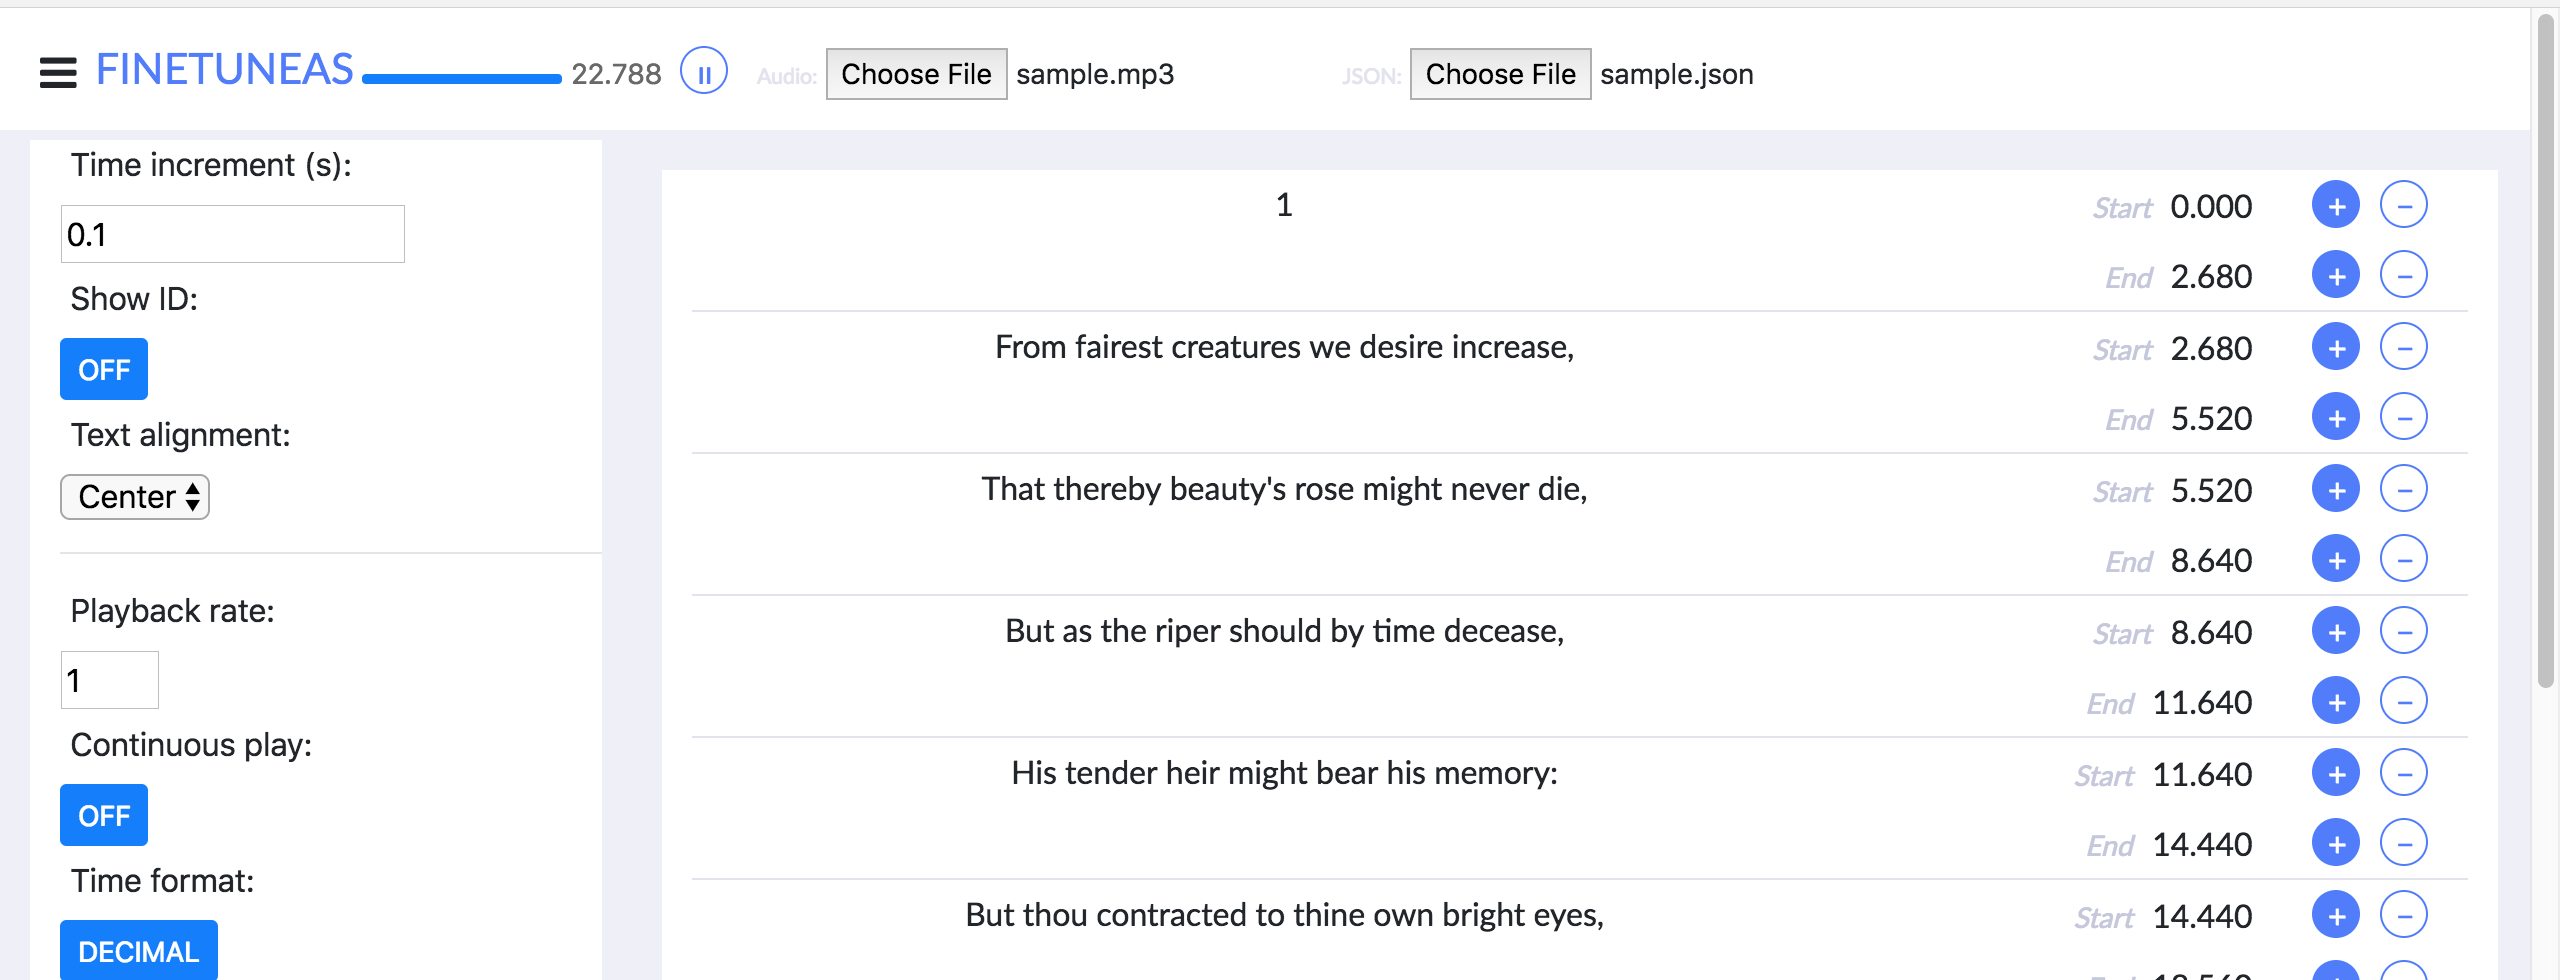
\includegraphics[width=\textwidth]{figures/finetuneas.png}
    \caption{Web interface van \texttt{finetuneas}}
    \label{fig:finetuneas}
\end{figure}


\section{Actorenanalyse}
\subsection{Ambities opdrachtgever}


%%%%%%%%%%%%%%%%%%%%%%%%%%%%%%%%%%%%%%%%%%%%%%%%%%%%%%%%%%%%%%%%%%%%%%%%

\section{Conclusies ontwikkelpotentie}
%%%%%%%%%%%%%%%%%%%%%%%%%%%%%%%%%%%%%%%%%%%%%%%%%%%%%%%%%%%%%%%%%%%%%%%%


